\section{Modello funzionale}
In questa sezione andremo a descrivere il modello funzionale del software
partendo da un analisi dei casi d'uso assegnati per l'applicativo, e proseguendo poi con tabelle cockburn e mock-up.
\subsection{Requisiti del software}
Lo sviluppo di Ratatouille23\texttrademark\ in parte è stato scandito dalla presenza di requisiti imposti dal cliente per il corretto funzionamento del software, in parte da requisiti tecnologici.

\subsubsection{Requisiti funzionali}
Il sistema offre le seguenti funzionalità:
\begin{enumerate}
  \item La possibilità da parte di un amministratore di poter creare utenze per i propri dipendenti (e.g. addetti alla sala, addetti alla cucina, supervisori) con nome utente scelto dall'aministratore ed una password di default.

  \item La possibilità da parte di un amministratore (o un supervisore) di personalizzare il menù dell'attività di ristorazione. In particolare, la possibilità di riordinare il menù, creare e/o eliminare elementi dal menù, caratterizzandoli tramite:
        \begin{itemize}
          \item \textit{nome}.
          \item \textit{descrizione}.
          \item \textit{elenco di allergeni comuni}.
          \item \textit{prezzo}.
        \end{itemize}
        In fase di creazione di un determinato piatto, è disponibile, utilizzando l'apposito tasto per la ricerca, l'autocompletamento di alcuni prodotti (e.g.: bibite o preconfezionati).
  \item La possibilità da parte di un addetto alla sala di poter registrare ordinazioni indicando l'identificativo del tavolo e gli elementi del menù (già presenti) desiderati.
  \item Un supervisore o un amministratore può inserire nel sistema degli avvisi (chiamati notifiche), che possono essere
        visualizzati da tutti i dipendenti. Ciascun dipendente può poi , qualora lo ritenesse necessario, marcare un avviso come “visualizzato” nascondendolo.
\end{enumerate}

\subsection{Requisiti non funzionali}
Le modalità secondo le quali saranno offerte le funzionalità sopracitate sono le seguenti:
\begin{itemize}
  \item \textbf{Usabilità} L'applicazione è stata sottoposta a una ricerca nel dettaglio di
        "User Personas" e monitoraggio tramite servizi official Google.inc.
  \item \textbf{Scalabilità}
        Scalabilità Il sistema deve avere un back-end in cloud scalabile per adat-
        tarsi a frequenze di accesso elevate.
  \item \textbf{Password policy security} Le password dell'utente verrano salvate in
        cloud con un controllo regex avanzato (vedesi testing) e sicurezza su crit-
        tografia SHA-256.
  \item \textbf{Utilizzo di single-activity, multi-fragment} L'applicazione utilizza per
        fluidità e facile gestione il pattern di single-activity e multi-fragment in modo
        da dare precisi scopi alle activity che gestiscono fragment comuni.
\end{itemize}
\subsection{Requisiti di dominio}
\begin{itemize}
  \item \textbf{ISO/IEC} Il sistema deve essere conforme alle direttive \textit{ISO/IEC} del trattamento dei dati privati su servizi di hosting in cloud.
  \item \textbf{GDPR} Il sistema segue le direttive euorpee sulla \textit{GDPR} e quelle delle policy della privacy.
\end{itemize}
\subsection{Descrizione use-case}
Di seguito sono descritti in dettaglio gli use-case scelti dal team di sviluppatori, al fine di dare un'idea concreta e chiara sul funzionamento del software sviluppato.
\subsubsection{Use-case generale}
Questo use-case è nato dopo aver attentamente valutato le richieste da parte degli stakeholders, infatti tale use-case contiene tutte le funzionalità richieste, mostrate in maniera semplificate solo ed esclusivamente per dare un idea generale delle possibilità offerte dal software.
\begin{center}
  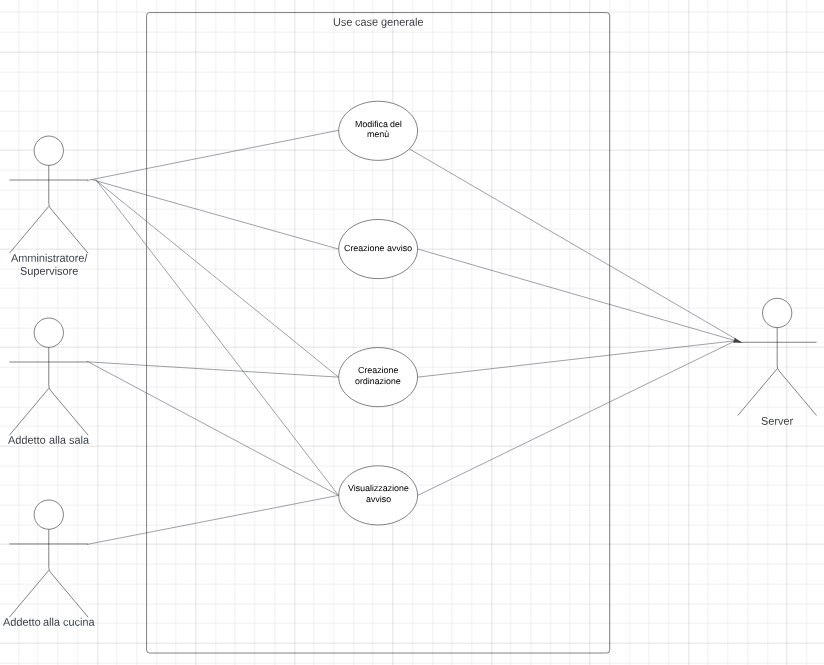
\includegraphics[scale=0.8]{img/use_case/use_case_generale.png}
\end{center}

\subsubsection{Creazione piatto}
La creazione del piatto è una delle funzionalità più elaborate, in quanto, non basterà essere un amministratore/supervisore e inserire i dati (nome, descrizione, allergeni, categoria e prezzo) necessari alla creazione di un piatto. Verrà infatti controllata l'esistenza del piatto e, nel caso di esito positivo il piatto non verrà creato, altrimenti verrà aggiunto alla categoria selezionata.
\begin{center}
  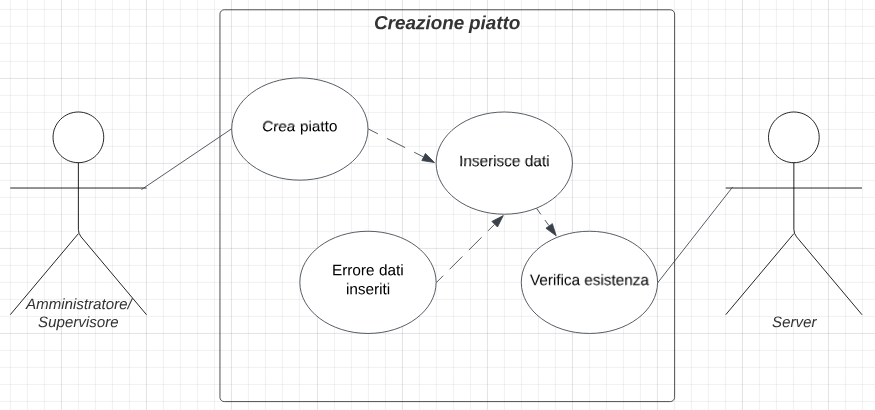
\includegraphics[scale=0.65]{img/use_case/use_case-creazione_piatto.png}
\end{center}
\subsubsection{Eliminazione piatto}
L'eliminazione del piatto è tutto sommato una funzionalità semplice ed autoesplicativa. Viene semplicemente scelto, da un amministratore/supervisore, il piatto che si desidera eliminare, una volta eliminato ci sarà una richiesta di conferma di eliminazione.
\begin{center}
  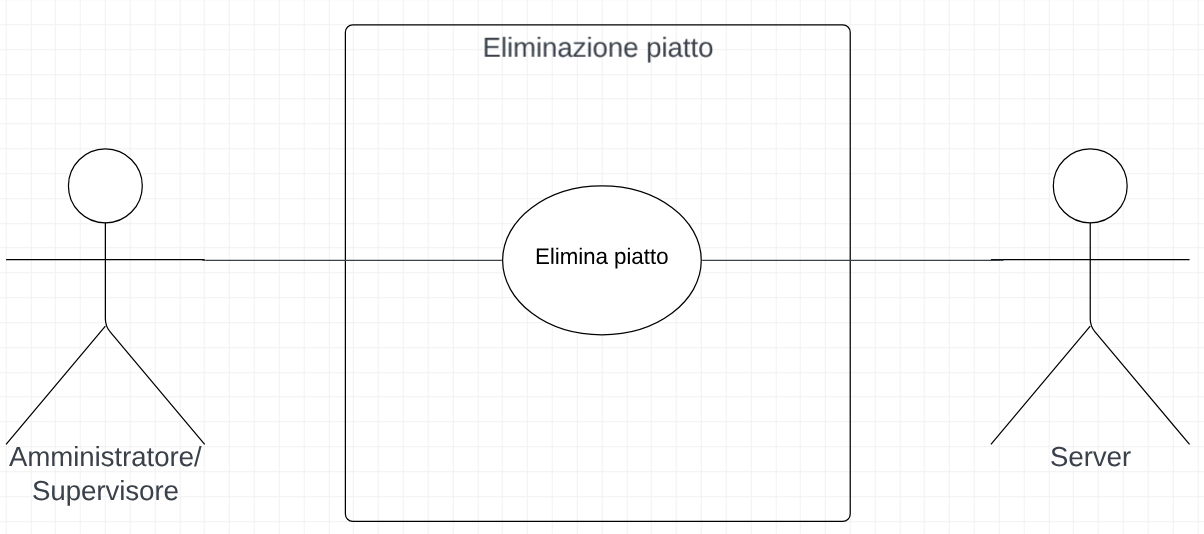
\includegraphics[scale=0.5]{img/use_case/use_case-eliminazione_piatto.png}
\end{center}
\newpage
\subsubsection{Creazione ordinazione}
La creazione di un ordinazione è un requistio fondamentale per la corretta gestione di un'attività di ristorazione che sia essa una tavola calda, un Autogrill o un classico risotrante. Per prima cosa è necessario che l'utente registrato che prova a creare un ordinazione è un "addetto alla sala". Infatti nel caso in cui l'utente registrato non appartiene a questa categoria, non gli sarà permesso a priori la creazione di un ordinazione. Per creare un ordinazione è necessario scegliere un tavolo (tramite l'identificativo associato), e selezionare i piatti che si vogliono aggiungere all'ordinazione (sarà possibile registrare più ordinazioni per lo stesso tavolo in momenti separati).
\begin{center}
  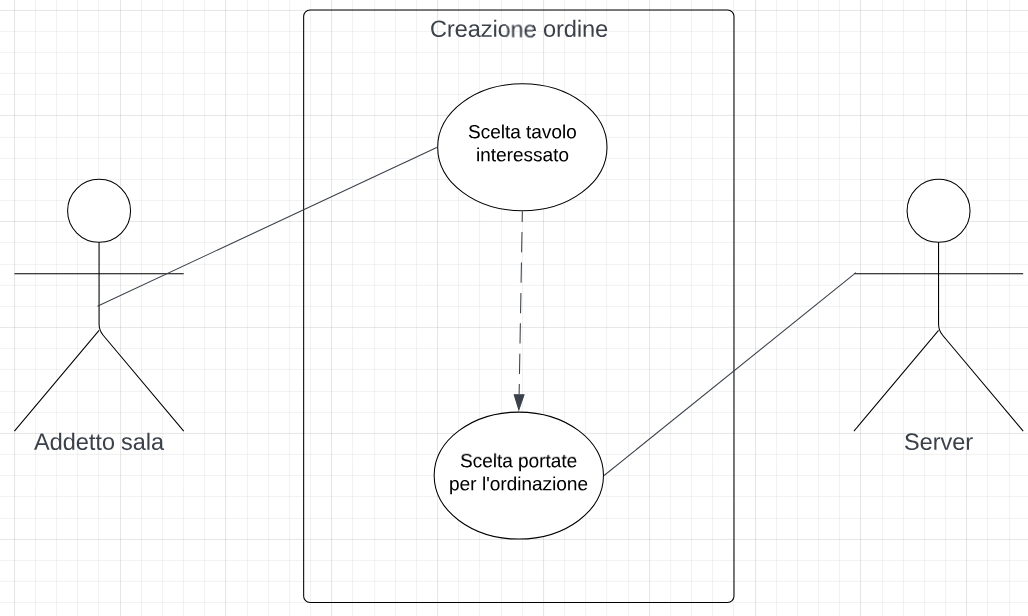
\includegraphics[scale=0.6]{img/use_case/use_case-creazione_ordine.png}
\end{center}
\newpage
\subsubsection{Creazione notifica}
La creazione di un avviso (notifica), è un aspetto fondamentale del software in quanto permette all'amministratore/supervisore di comunicare informazioni importanti indistintamente ad ogni utente. Infatti gli unici utenti con permessi per creare un avviso (notifica) sono proprio l'amministratore e i supervisori.
\begin{center}
  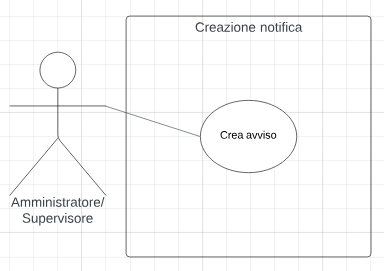
\includegraphics[scale=0.6]{img/use_case/use_case-creazione_notifica.png}
\end{center}
\newpage
\subsection{Tabelle cockburn}
Ci è stato richiesto di presentare, tra i casi d'uso assegnati, quattro casi
specifici a scelta descrivendoli tramite \textbf{tabelle di Cockburn}.
\paragraph{Cosa sono?} Le tabelle di Cockburn (create da \textit{Alistair Cockburn}, dal quale prendono il nome) sono un formalismo di rappresentazione dei casi d'uso.\\
La politica adotta la rappresentazione di un Main scenario nella quale uno o più attori interagiscono
tra loro attraverso l'invocazione di trigger e descrivendo (in formato tabellare) gli eventi.
\\
\\Per garantire una certa corenza al committente e una comprensione a tutto tondo abbiamo scelto gli stessi casi esplorati nella presentazione dei casi d'uso.
\subsubsection{Creazione Ordinazione}
\begin{table}[H]
  \def\arraystretch{1.5}
  \begin{tabularx}{\linewidth}{|l|X|X|X|}
    \hline \textbf{Use Case \#1}           & \multicolumn{3} {l|}{\textbf{Creazione ordinazione}}                                                                                                      \\ \hline \textbf{Goal in
    Context}                               & \multicolumn{3}{>{\hsize=\dimexpr 3\hsize+4\tabcolsep+2\arrayrulewidth\relax}X|}{                                                                         %
    L'addetto alla sala vuole creare una nuova ordinazione per un tavolo}                                                                                                                              \\
    \hline \textbf{Preconditions}          &
    \multicolumn{3}{l|}{L'addetto alla sala deve essersi autenticato correttamente}                                                                                                                    \\
    \hline \textbf{Success End Conditions} &
    \multicolumn{3}{l|}{La nuova ordinazione è stata creata}                                                                                                                                           \\
    \hline \textbf{Failed End Conditions}  &
    \multicolumn{3}{l|}{Le informazioni inserite non sono valide}                                                                                                                                      \\
    \hline \textbf{Primary Actor}          &
    \multicolumn{3}{l|}{Utente autenticato}                                                                                                                                                            \\
    \hline \textbf{Trigger}                & \multicolumn{3}{l|}{Pressione del tasto "crea ordinazione"}                                                                                               \\

    \hline \multirow{2}{*}{\textbf{Description}}
                                           & \textbf{Step}                                                                     & \textbf{Addetto sala}        & \textbf{Server}                        \\
    \cline{2-4}                            & 1                                                                                 & Sceglie il tavolo            &                                        \\
    \cline{2-4}                            & 2                                                                                 & Sceglie i piatti da inserire &                                        \\
    \cline{2-4}                            & 3                                                                                 & Conferma l'ordine            & Verifica esistenza del tavolo          \\
    \cline{2-4}                            & 4                                                                                 &                              & Verifica esistenza dei piatti inseriti \\

    \cline{2-4}                            & 5                                                                                 &                              & Registra ordine                        \\
    \hline
  \end{tabularx}
\end{table}
\subsubsection{Eliminazione piatto}
\begin{table}[H]
  \def\arraystretch{1.5}
  \begin{tabularx}{\linewidth}{|l|X|X|X|}
    \hline \textbf{Use Case \#2}                 & \multicolumn{3} {l|}{\textbf{Eliminazione piatto}}                                                                                       \\ \hline \textbf{Goal in
    Context}                                     & \multicolumn{3}{>{\hsize=\dimexpr 3\hsize+4\tabcolsep+2\arrayrulewidth\relax}X|}{                                                        %
    L'utente vuole eliminare un piatto dal menù}                                                                                                                                            \\
    \hline \textbf{Preconditions}                &
    \multicolumn{3}{l|}{L'utente è autenticato correttamente ed ha i permessi}                                                                                                              \\
    \hline \textbf{Success End Conditions}       &
    \multicolumn{3}{l|}{Il piatto è stato eliminato}                                                                                                                                        \\
    \hline \textbf{Failed End Conditions}        &
    \multicolumn{3}{l|}{Il piatto che ha provato ad eliminare non è valido}                                                                                                                 \\
    \hline \textbf{Primary Actor}                &
    \multicolumn{3}{l|}{Amministratore/supervisore}                                                                                                                                         \\
    \hline \textbf{Trigger}                      & \multicolumn{3}{l|}{Pressione tasto "elimina piatto"}                                                                                    \\

    \hline \multirow{2}{*}{\textbf{Description}} & \textbf{Step}                                                                     &
    \textbf{Client}                              & \textbf{Server}                                                                                                                          \\
    \cline{2-4}                                  & 1                                                                                 & Seleziona il piatto da eliminare &                   \\
    \cline{2-4}                                  & 2                                                                                 & Apertura dialog di conferma      &                   \\
    \cline{2-4}                                  & 3                                                                                 & Conferma l'eliminazione          &                   \\
    \cline{2-4}                                  & 4                                                                                 &                                  & Elimina il piatto \\
    \hline
  \end{tabularx}
\end{table}

\subsubsection{Creazione piatto}
\begin{table}[H]
  \def\arraystretch{1.5}
  \begin{tabularx}{\linewidth}{|l|X|X|X|}
    \hline \textbf{Use Case \#3}                 & \multicolumn{3} {l|}{\textbf{Creazione piatto}}                                                                                                                                                                                            \\ \hline \textbf{Goal in
    Context}                                     & \multicolumn{3}{>{\hsize=\dimexpr 3\hsize+4\tabcolsep+2\arrayrulewidth\relax}X|}{L'utente vuole creare un piatto da aggiungere al menù}                                                                                                    \\
    \hline \textbf{Preconditions}                &
    \multicolumn{3}{l|}{L'utente è collegato correttamente ed ha i permessi necessari}                                                                                                                                                                                                        \\
    \hline \textbf{Success End Conditions}       &
    \multicolumn{3}{l|}{Il piatto è stato creato}                                                                                                                                                                                                                                             \\
    \hline \textbf{Failed End Conditions}        &
    \multicolumn{3}{l|}{Le informazioni inserite sono già presenti o non valide}                                                                                                                                                                                                              \\
    \hline \textbf{Primary Actor}                &
    \multicolumn{3}{l|}{Amministratore/supervisore}                                                                                                                                                                                                                                           \\
    \hline \textbf{Trigger}                      & \multicolumn{3}{l|}{Apertura schermata creazione piatto}                                                                                                                                                                                   \\

    \hline \multirow{2}{*}{\textbf{Description}} & \textbf{Step}                                                                                                                           &
    \textbf{Client}                              & \textbf{Server}                                                                                                                                                                                                                            \\
    \cline{2-4}                                  & 1                                                                                                                                       & Inserisce i dati richiesti per la creazione &                                                    \\
    \cline{2-4}                                  & 2                                                                                                                                       & Clicca tasto "crea piatto"                  &                                                    \\
    \cline{2-4}                                  & 3                                                                                                                                       &                                             & Verifica la possibilità della creazione del piatto \\
    \cline{2-4}                                  & 4                                                                                                                                       &                                             & Salva il piatto                                    \\
    \hline
  \end{tabularx}
\end{table}
\subsubsection{Creazione notifica}
\begin{table}[H]
  \def\arraystretch{1.5}
  \begin{tabularx}{\linewidth}{|l|X|X|X|}
    \hline \textbf{Use Case \#4}                 & \multicolumn{3} {l|}{\textbf{Creazione notifica}}                                                                                                                           \\ \hline \textbf{Goal in
    Context}                                     & \multicolumn{3}{>{\hsize=\dimexpr 3\hsize+4\tabcolsep+2\arrayrulewidth\relax}X|}{                                                                                           %
    L'utente vuole creare una notifica da inviare ai dipendenti}                                                                                                                                                               \\
    \hline \textbf{Preconditions}                &
    \multicolumn{3}{l|}{L'utente è autenticato correttamente ed ha i permessi}                                                                                                                                                 \\
    \hline \textbf{Success End Conditions}       &
    \multicolumn{3}{l|}{La notifica è stata creata}                                                                                                                                                                            \\
    \hline \textbf{Failed End Conditions}        &
    \multicolumn{3}{l|}{La notifica con la stessa data è già presente}                                                                                                                                                         \\
    \hline \textbf{Primary Actor}                &
    \multicolumn{3}{l|}{Amministratore/supervisore}                                                                                                                                                                            \\
    \hline \textbf{Trigger}                      & \multicolumn{3}{l|}{Pressione tasto "crea notifica"}                                                                                                                        \\

    \hline \multirow{2}{*}{\textbf{Description}} & \textbf{Step}                                                                     &
    \textbf{Client}                              & \textbf{Server}                                                                                                                                                             \\
    \cline{2-4}                                  & 1                                                                                 & Inserisce titolo e testo della notifica    &                                            \\
    \cline{2-4}                                  & 2                                                                                 & Preme il tasto per confermare la creazione & Verifica se la notifica non è già presente \\
    \cline{2-4}                                  & 3                                                                                 &                                            & Salva la notifica                          \\
    \hline
  \end{tabularx}

\end{table}
\newpage
\subsection{Mock-Up}
Un mock-up , è una realizzazione a scopo illustrativo o meramente espositivo, di un oggetto o un sistema, senza le complete funzioni
dell'originale; un mockup può rappresentare la totalità o solo una parte dell'originale di riferimento (già esistente o in fase di progetto), essere in scala
reale oppure variata.
\begin{center}
  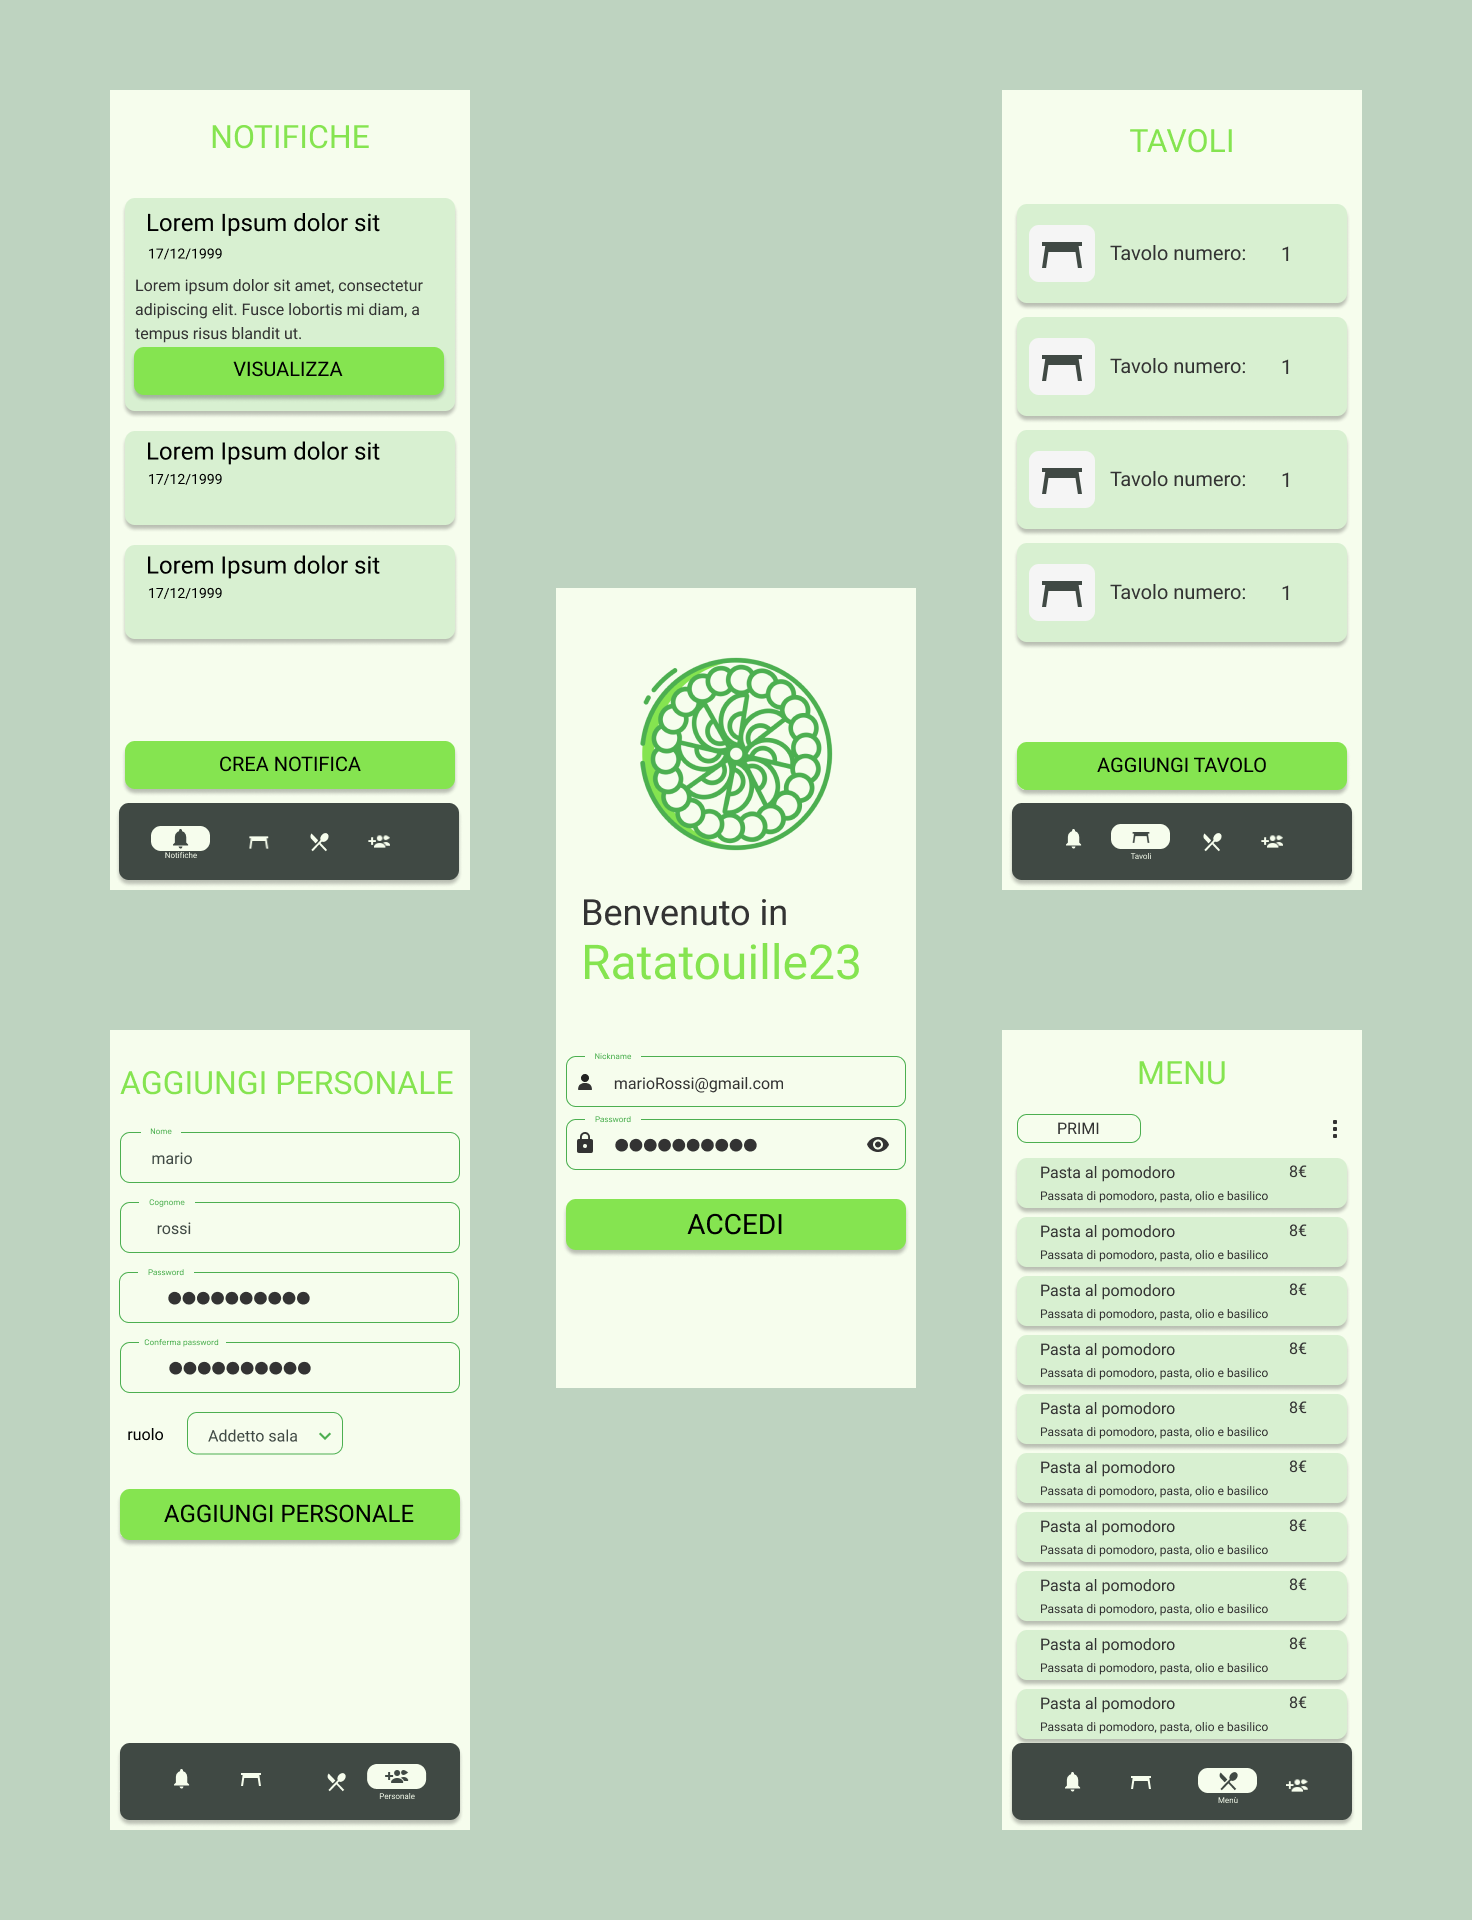
\includegraphics[scale=0.2]{img/Mock-up.doc}
\end{center}
La versione del mock-up qui sopra rappresenta le schermate principali dell'applicazione. Nella realizzazione di quest'applicazione c'è stato uno studio del colore e dell'usabilità, con una palette creata appositamente per non stancare gli occhi e rendere il tutto più "vicino" al cibo possibile.\\
Di seguito andremo a visualizzare i mock-up dei metodi scelti dal team.
\subsubsection{Creazione piatto}
\subsubsection{Eliminazione piatto}
\subsubsection{Creazione ordinazione}
\subsubsection{Creazione notifica}